
\section{Model with phases} \label{sec:model_with_phases}

The energy efficiency of HPC can be achieved through dynamic workload planning. Dynamic scaling of frequency and voltage DVFS is the main energy efficiency technique to save power. The scaling algorithms can operate dynamically depending on the CPU workload. However, the required IT resources and workload vary throughout the applications' execution. The division of this workload directly impacts the resulting performance and the complexity of dynamic scaling algorithms. This work analyses the impact on the energy efficiency of different dynamic workload partitioning techniques, based on time division of allocated resources and DVFS. We evaluate the trade-off between the best time intervals partition and the overhead impact of dynamic scheduling techniques. We propose the optimal partition of application executions in time intervals providing the most energy efficient execution parameters, workload, frequency and number of cores, for each time interval.

\section{Introduction to models on time} \label{sec:introduction_to_models_on_time}
Talk about the importance of energy efficiency.

\section{Phases related work} \label{sec:related_work_phases}
Some related work

\section{Optimal energy configuration} \label{sec:Optimal_energy_configuration}
Splitting a program into phases, or time intervals with a selected set of execution parameters, has an impact on energy consumption. To find the ideal phase division, we need to compute the optimal energy configuration for a given number and duration of phases. For that, many different approaches could be applied, each having different trade-offs. 

Using models ref [x], or a static analysis of the application, allows obtaining a very fast but less precise estimate. On the other hand, using the application and evaluating its behavior in each possible context would be a more reliable but too expensive method. Indeed, since the number of combinations grows exponentially, this is a very time consuming approach. Instead, our analysis approach will provide both, speed and precision. We will simply run the target application and collect performance data from every possible execution context. By context, we can consider, for instance, the frequency and/or number of cores. This data will then be used to analyse the behavior of phases in all possible combinations. For this, we assume that the number of instructions of the executed program is the same regardless of frequency and number of threads.

\begin{equation}
    I=c_{k1}f_1T_1=c_{k2}f_2T_2
\end{equation}

where $I$ is the number of instructions, $c_{k1}$ the rate of instructions per cycle, $f$ the frequency of the processor and $T$ the execution time. All the required parameters can be collected by simply running the application with the available frequencies. 

From this equation we can split the execution of the program into several different phases $i$ as follows:
% \begin{equation}
%     I=xI+(1-x)I=xc_{k1}f_1+(1-x)c_{k2}f_2
% \end{equation}
\begin{equation}
    I=\sum_{i}{a_iI} %=\sum_i{a_ic_{ki}f_i}
\end{equation}

with $a_i$ as the percentages of instructions executed with frequency $f_i$, we can compute any combination of phases. For convenience, we write this as a function of the time:
% \begin{equation}
% T=\frac{I}{c_{k1}f_1}
% \end{equation}
\begin{equation}
I=Tc_{k}f
\end{equation}
\begin{equation}
    I=\sum_{i}{a_iI}=\sum_i{a_iTc_{ki}f_i}
\end{equation}
% \begin{equation}
% I=xI+(1-x)I=xTc_{k1}f_1+(1-x)Tc_{k2}f_2
% \end{equation}

the application being divided into phases of different duration, $a_i$  becomes the duration of the phase as a percentage of the total execution time. This general equation does not limit the number and duration of phases, and several phases can have the same frequency. 

In the event that we decide to include the number of cores as a context parameter, the equation becomes more complex. Indeed, the number of cores can completely change the application's behavior but, depending on the type of application, it's still possible to find similarities. Many HPC applications use data parallelism, and the Amdahl's law can model most of it. For this kind of applications, we can estimate that:
\begin{equation}
T=\frac{T_s}{S}
\end{equation}
\begin{equation}
T_s=\frac{I}{c_kf}
\end{equation}
\begin{equation}
S=\frac{1}{1-w+\frac{w}{p}}
\end{equation}
\begin{equation}
T=\frac{I(1-w+\frac{w}{p})}{c_kf}=\frac{I}{c_kf}-\frac{Iw}{c_kf}+\frac{Iw}{c_kfp}
\end{equation}


Looking at a fixed frequency, we arrive at a very similar structure as before:
\begin{equation}
T=c_1I+\frac{c_2I}{p}
\end{equation}


As previously, we can use $I$ as the number of reference instructions, and compute $a$ as the percentage of single and multi-core instructions, or express it as a percentage of the total time T:
\begin{equation}
aT=c_1aI+\frac{c_2aI}{p}
\end{equation}


The extent of the hypotheses will later be validated, however, by taking advantage of both principles, we can now, based on real measurements, estimate any phase division and possible context combination.


% Here a need to show that the time is proportional to the number of executed instructions.
% WHY ?
% I am trying to say here that we can split the program using a percentage of the time because the time is proportional to the number of executed instructions. If we complete x% of the time, that will be x% of instructions. This implies that we can resume and continue the program from any point ensuring that we executed all instructions. If we have a previous execution for each configuration, we can compute any combination with minimal error.


\section{Data collection} \label{sec:data_collection}
Data, power samples, can be gathered by running the application in several possible context configurations. In a system with 32 cores that can run at 13 frequencies, we can have 416 (32*13) possible configurations. Power samples can be taken from dedicated sensors in the IPMI system [REF]. To avoid overload, a sample rate of 0.5 seconds is more than sufficient. Additionally, the behavior of an application can be affected by the workload, so it is also interesting to run applications with different inputs and assess their impact on the collected data [REF victor alex paper].

% We can consider different input sizes as an new application...

\section{The simulator} \label{sec:the_simulator}
To analyse the impact of configurations and identify optimal time-intervals, phases, we propose an integrator, which computes the energy on an interval for a given configuration, and a reference, a brute force test of all possible combinations. The integrator has order zero, and computers the energy between two timestamps, as shown in the figure \ref{fig:zero_order}, where the red and yellow parts area are the energy value.


\begin{figure}[H]
    \centering
    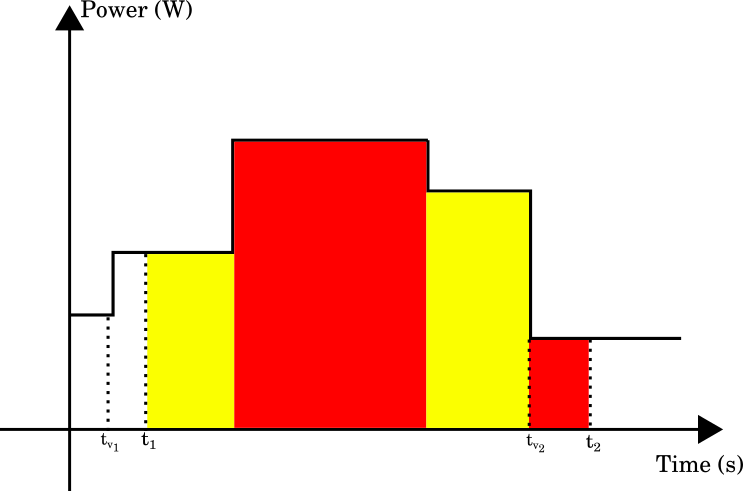
\includegraphics[width=\columnwidth]{phases/figures/zero_order.png}
    \caption{Power vs time intervals for a given application. The energy associated area is colored.}
    \label{fig:zero_order}
\end{figure}

Power and energy can be computed for a given time interval based on power samples. The pseudo-algorithm for this computation is described bellow:

\begin{lstlisting}
timeslice_energy(info, start, stop)
{
   power = info.power;
   time = info.time;
   
   t1 = start_time + (elapsed_time) * start;
   t2 = start_time + (elapsed_time) * stop;
   en = 0;

   // first time that is greater than t1
   for(i=0; i<nsamples; i++)
       if(time[i] >= t1)
           break;
   v1 = (i == 0)?0:i-1;
   // first time that is greater than t2
   for(i=v1; i<nsamples; i++)
       if(time[i] >= t2)
           break;
   v2 = (i == 0)?0:i-1;
 
   // interpolate and integrates the power samples
   if(v1 == v2)
       return (t2-t1)*power[v1];
 
   en = (time[v1+1]-t1)*power[v1];
   en += (t2-time[v2])*power[v2];
   // integrate samples in between
   for(i=v1+1; i<v2; i++)
       en += (time[i+1]-time[i])*power[i];
   return en;
}
\end{lstlisting}

The reference can simply be obtained by applying brute-force, which cycles through all configurations for all divisions and compute the minimal energy. Other more effective, but less accurate, methods can be applied.

\begin{lstlisting}
bruteforce(data, phases)
{
   min_en = -1;
   total_en = 0;
   for (i = 0; i < nphases; i++)
   {
       min_en = -1;
       for (j = 0; j<data.nconfigs; j++)
       {
           en = timeslice_energy(data.info[j], 
                        phases[i], phases[i + 1]);
           if (min_en == -1 || en < min_en)
           {
               min_en = en;
               min_conf = data.config[j];
           }
       }
       total_en += min_en;
   }
   return total_en;
}
\end{lstlisting}

\section{Optimizing phases} \label{sec:optimizing_phases}
The main goal of this section is to identify the optimal number and duration of time intervals. Indeed, several short phases can have an impact on switching overhead as well as few long phases on the overall energy. 

Using the objective function, brute force can identify the optimal energy on each phase and any minimization method can provide the best phase division. By computing in a range of a number of phases, we can find the one that brings the lowest energy value. A genetic algorithm GA can be used to analyse a range of, for instance, 3 to 100 phases. A GA for a population of 10K individuals with a 0.1 elitism will ensure that 10\% of the best individuals will survive and 0.1 mutations will avoid local minimums within a maximum of 300 steps. A reproduction function will combine the half-phases of one individual with another, and the mutation will randomly change a division.

\section{Phases experiments results} \label{sec:results_phases_experiments}

% Normalization
% Show that number of instructions is the same...

In order to validate the approach, HPC benchmarks where chosen, 13 applications from PARSEC 3.0, HPC, and Openmc.

\begin{figure}[H]
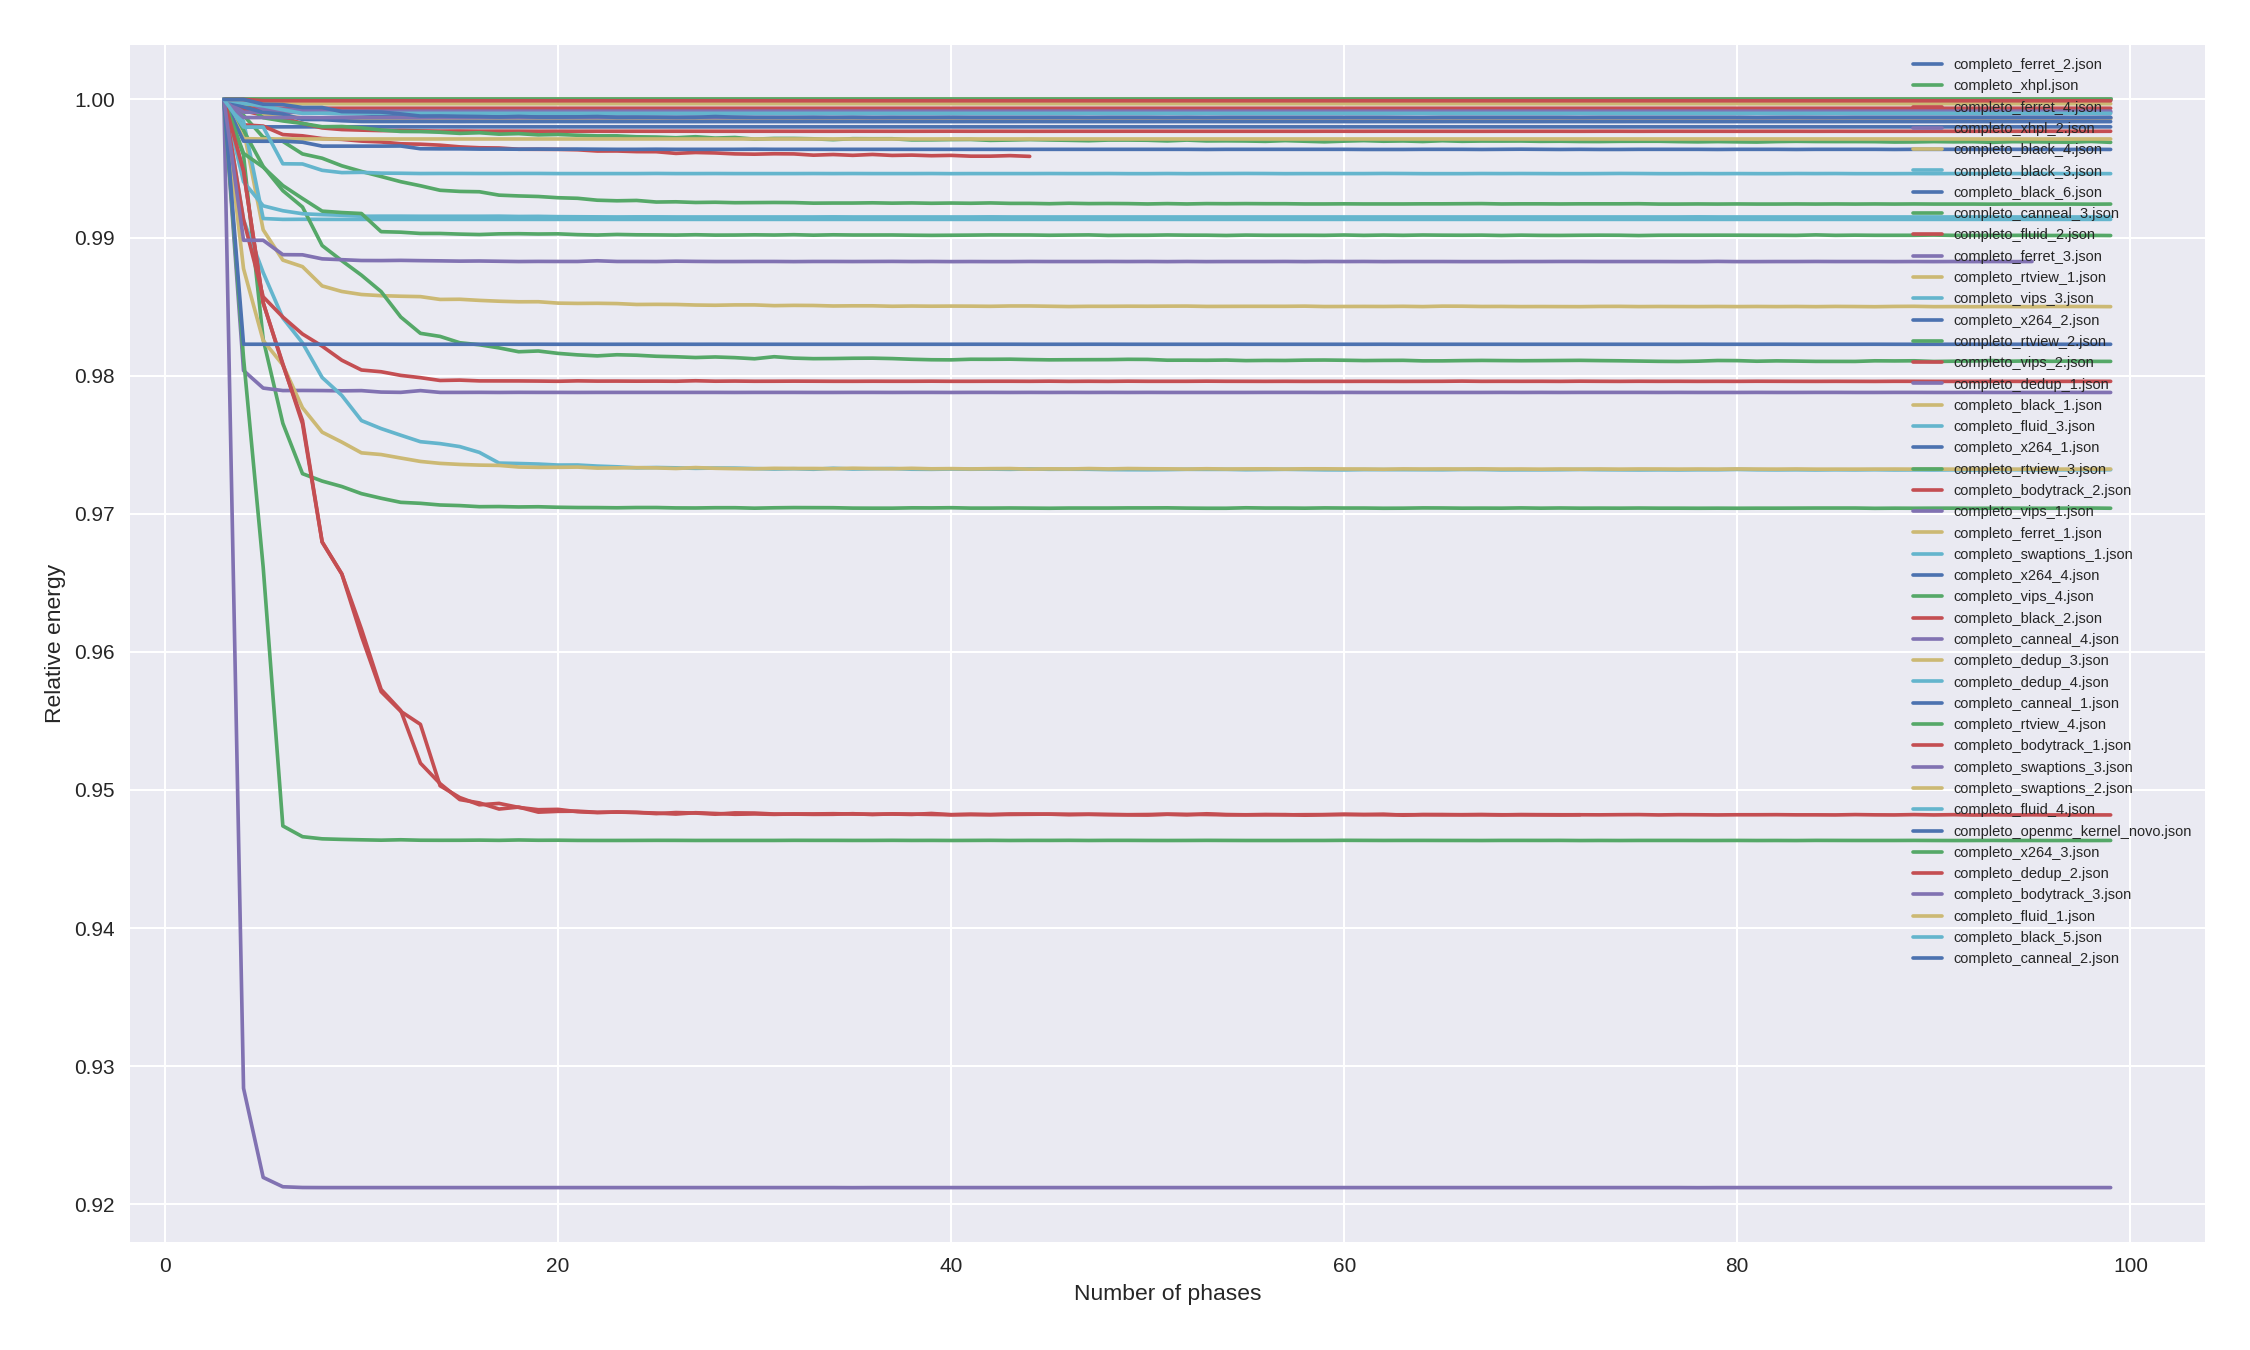
\includegraphics[width=\columnwidth]{fingerprint/figures/energy_per_phase.png}
    \caption{Relative energy vs number of phases using 13 applications from PARSEC 3.0, HPC, and Openmc benchmarks. Energy compared to the single-phase optimal configuration.}
    \label{fig:relative_energy}
\end{figure}

This evaluation shows very interesting results, as shown in the figure \ref{fig:relative_energy}. Indeed, for all cases, an optimal single-phase configuration gives the highest energy draw. On the contrary, it is not necessary to split the application into more than 35 phases. On average, the energy consumption stood still after 35 phases. 

The results attend our expectation that the optimal with n divisions will always be better or equal than n-1 divisions. This can be explained by the fact that after we find the ideal frequency and core curves, increasing the number of phases will not change the control signals. Therefore the energy will remain the same, and there is no reason to increase the number of phases beyond that actually. 

It is important to note that the additional energy savings that theoretically may be achieved when running with a greater number of phases will have a negative impact on performance and context switching. Moreover, the maximal energy saving compared to the single-phase case was just 2.6\%. This may be due to the type of applications, where a fine-grain fast control will not save more energy. On the contrary, this switching will cause to consume a lot more energy, and this is likely to happen with online DVFS algorithms, very sensitive to fast workload variations [REF].

We evaluated separately the impact on energy when varying the number of cores. Energy-cores figures doesn't change fundamentally varying the number of phases. Indeed, bellow we can see some examples with optimal energy cores selections for 60 and 70 phases (figure \ref{fig:cores_control}). Note the very small differences that will not change significantly the energy figures.

\begin{figure}[h!]
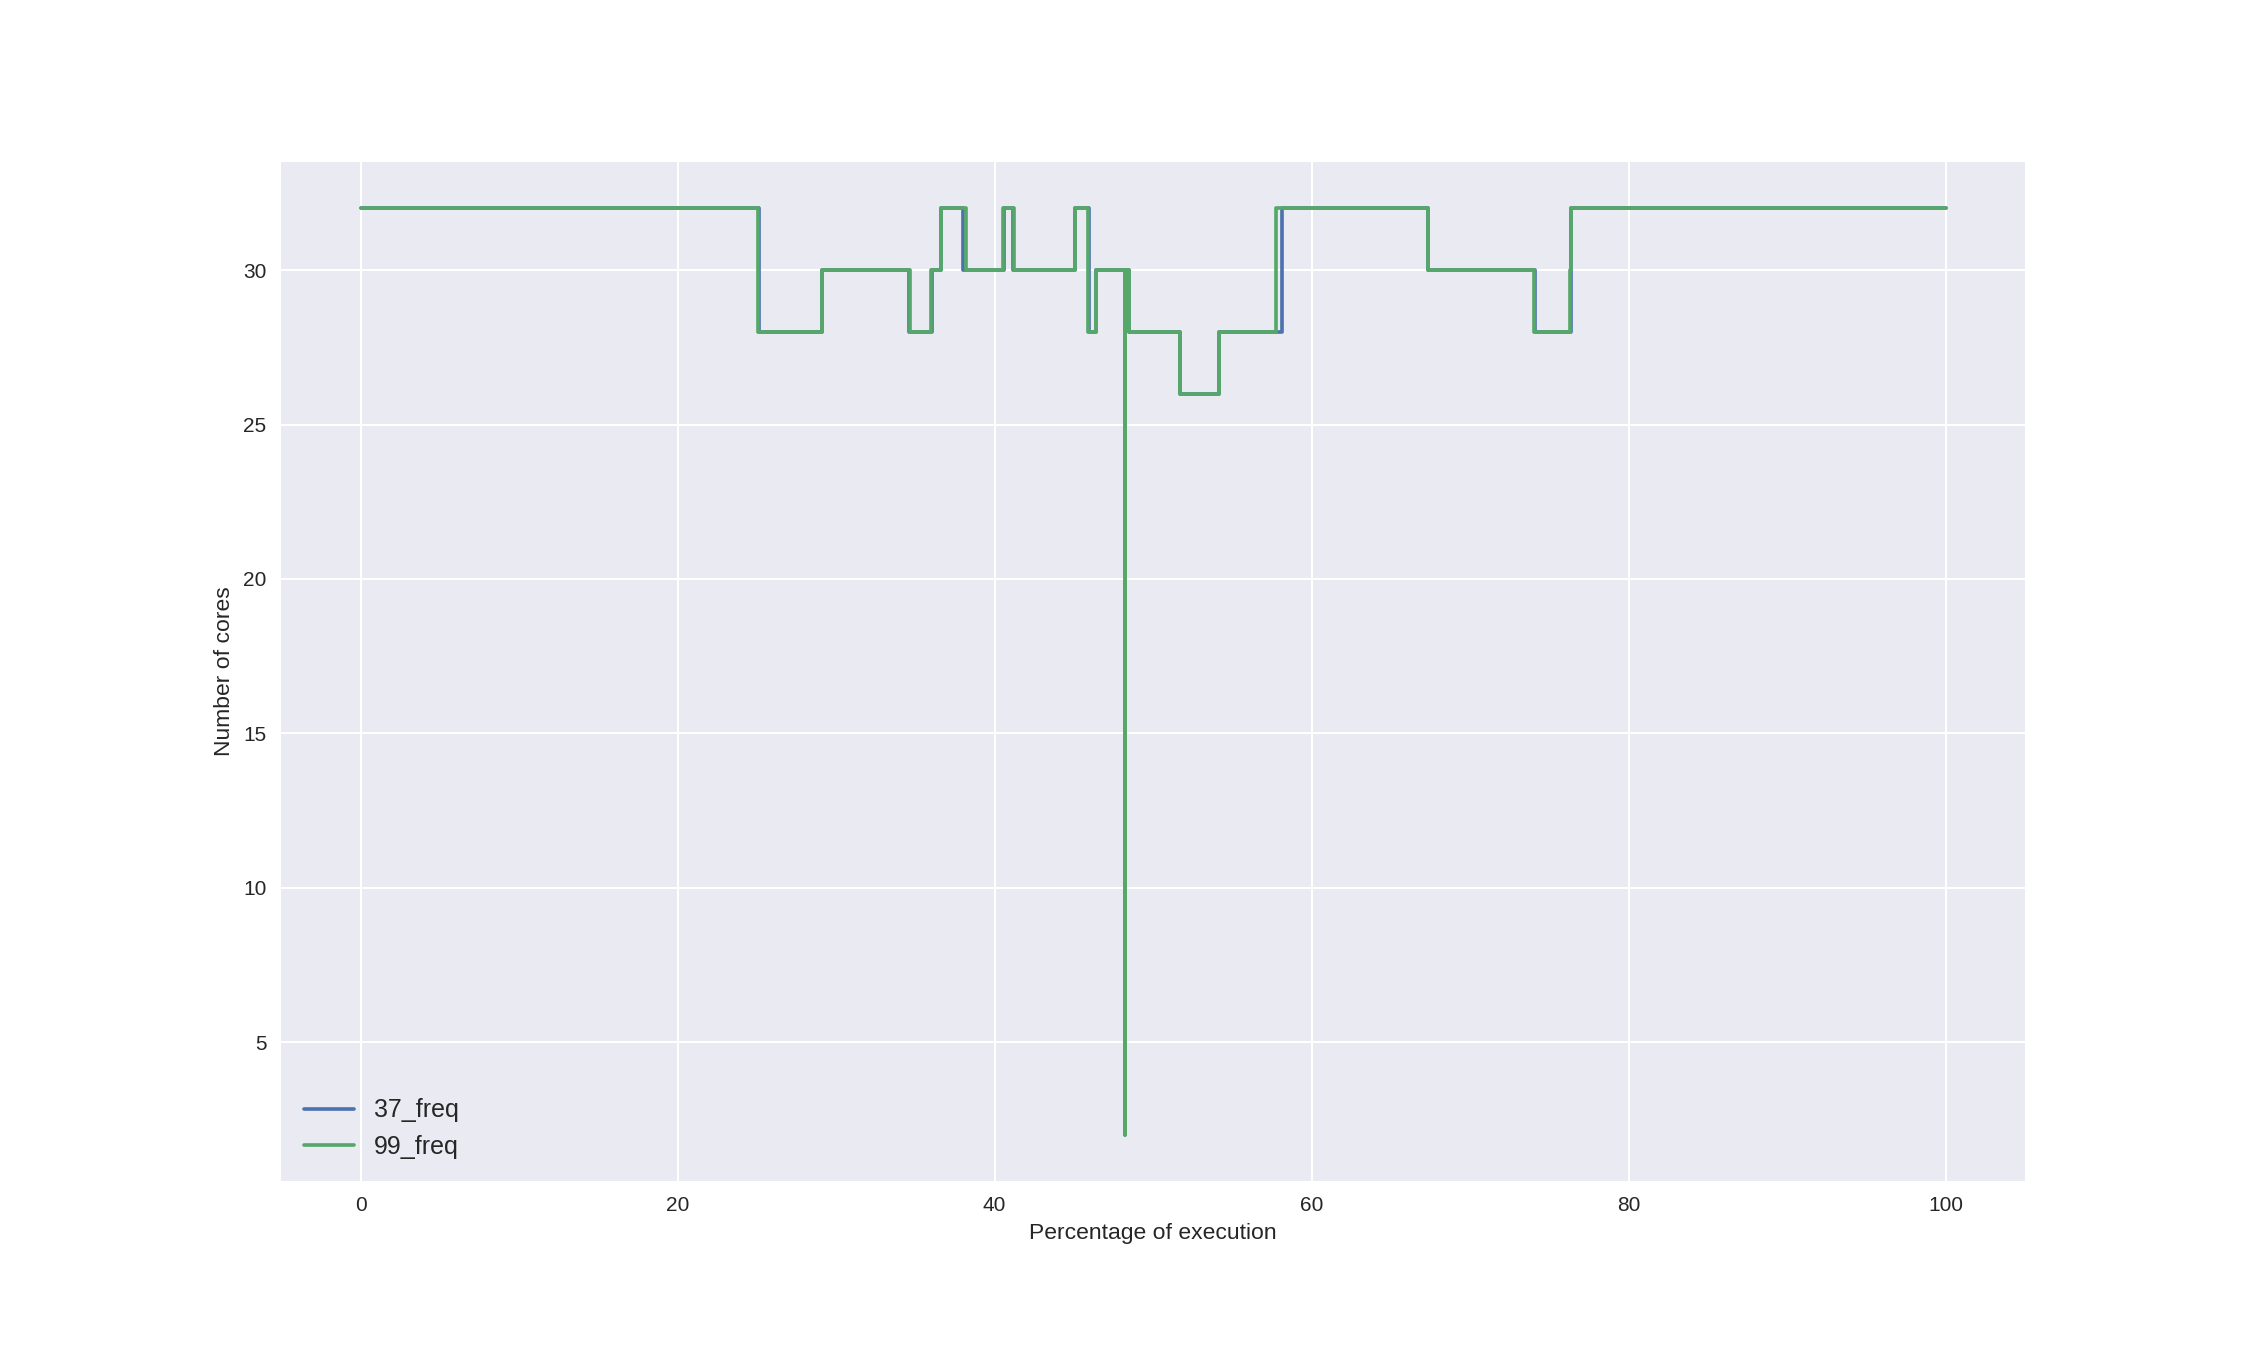
\includegraphics[width=\columnwidth]{phases/figures/signals/completo_black_3_cores_signals_cmp.png}
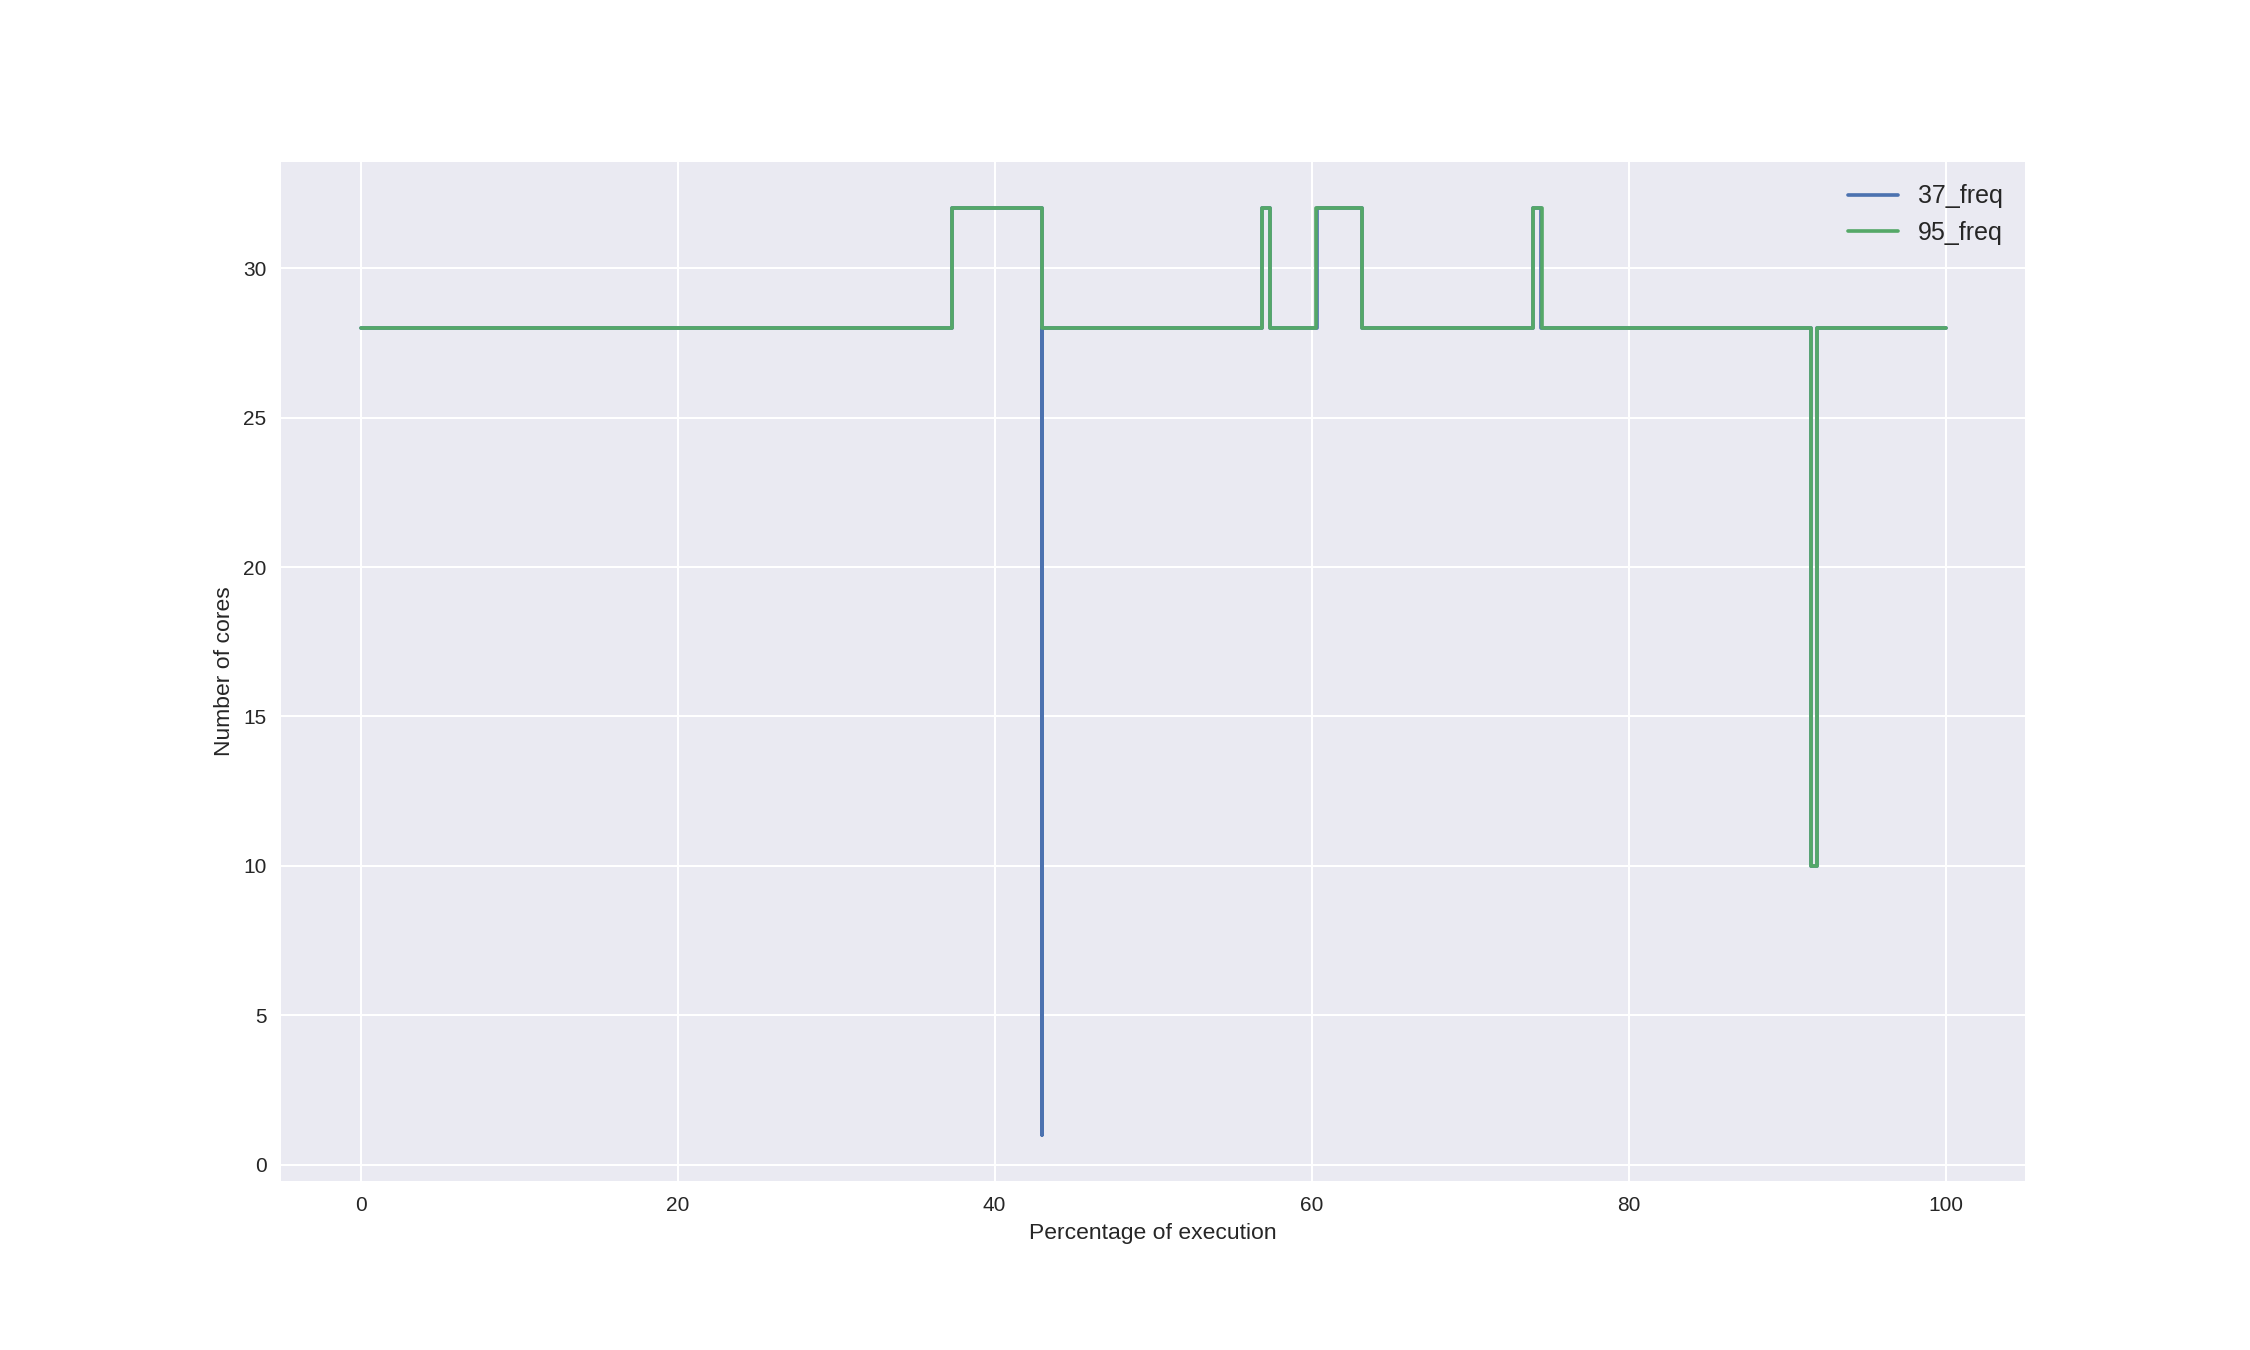
\includegraphics[width=\columnwidth]{phases/figures/signals/completo_bodytrack_3_cores_signals_cmp.png}
%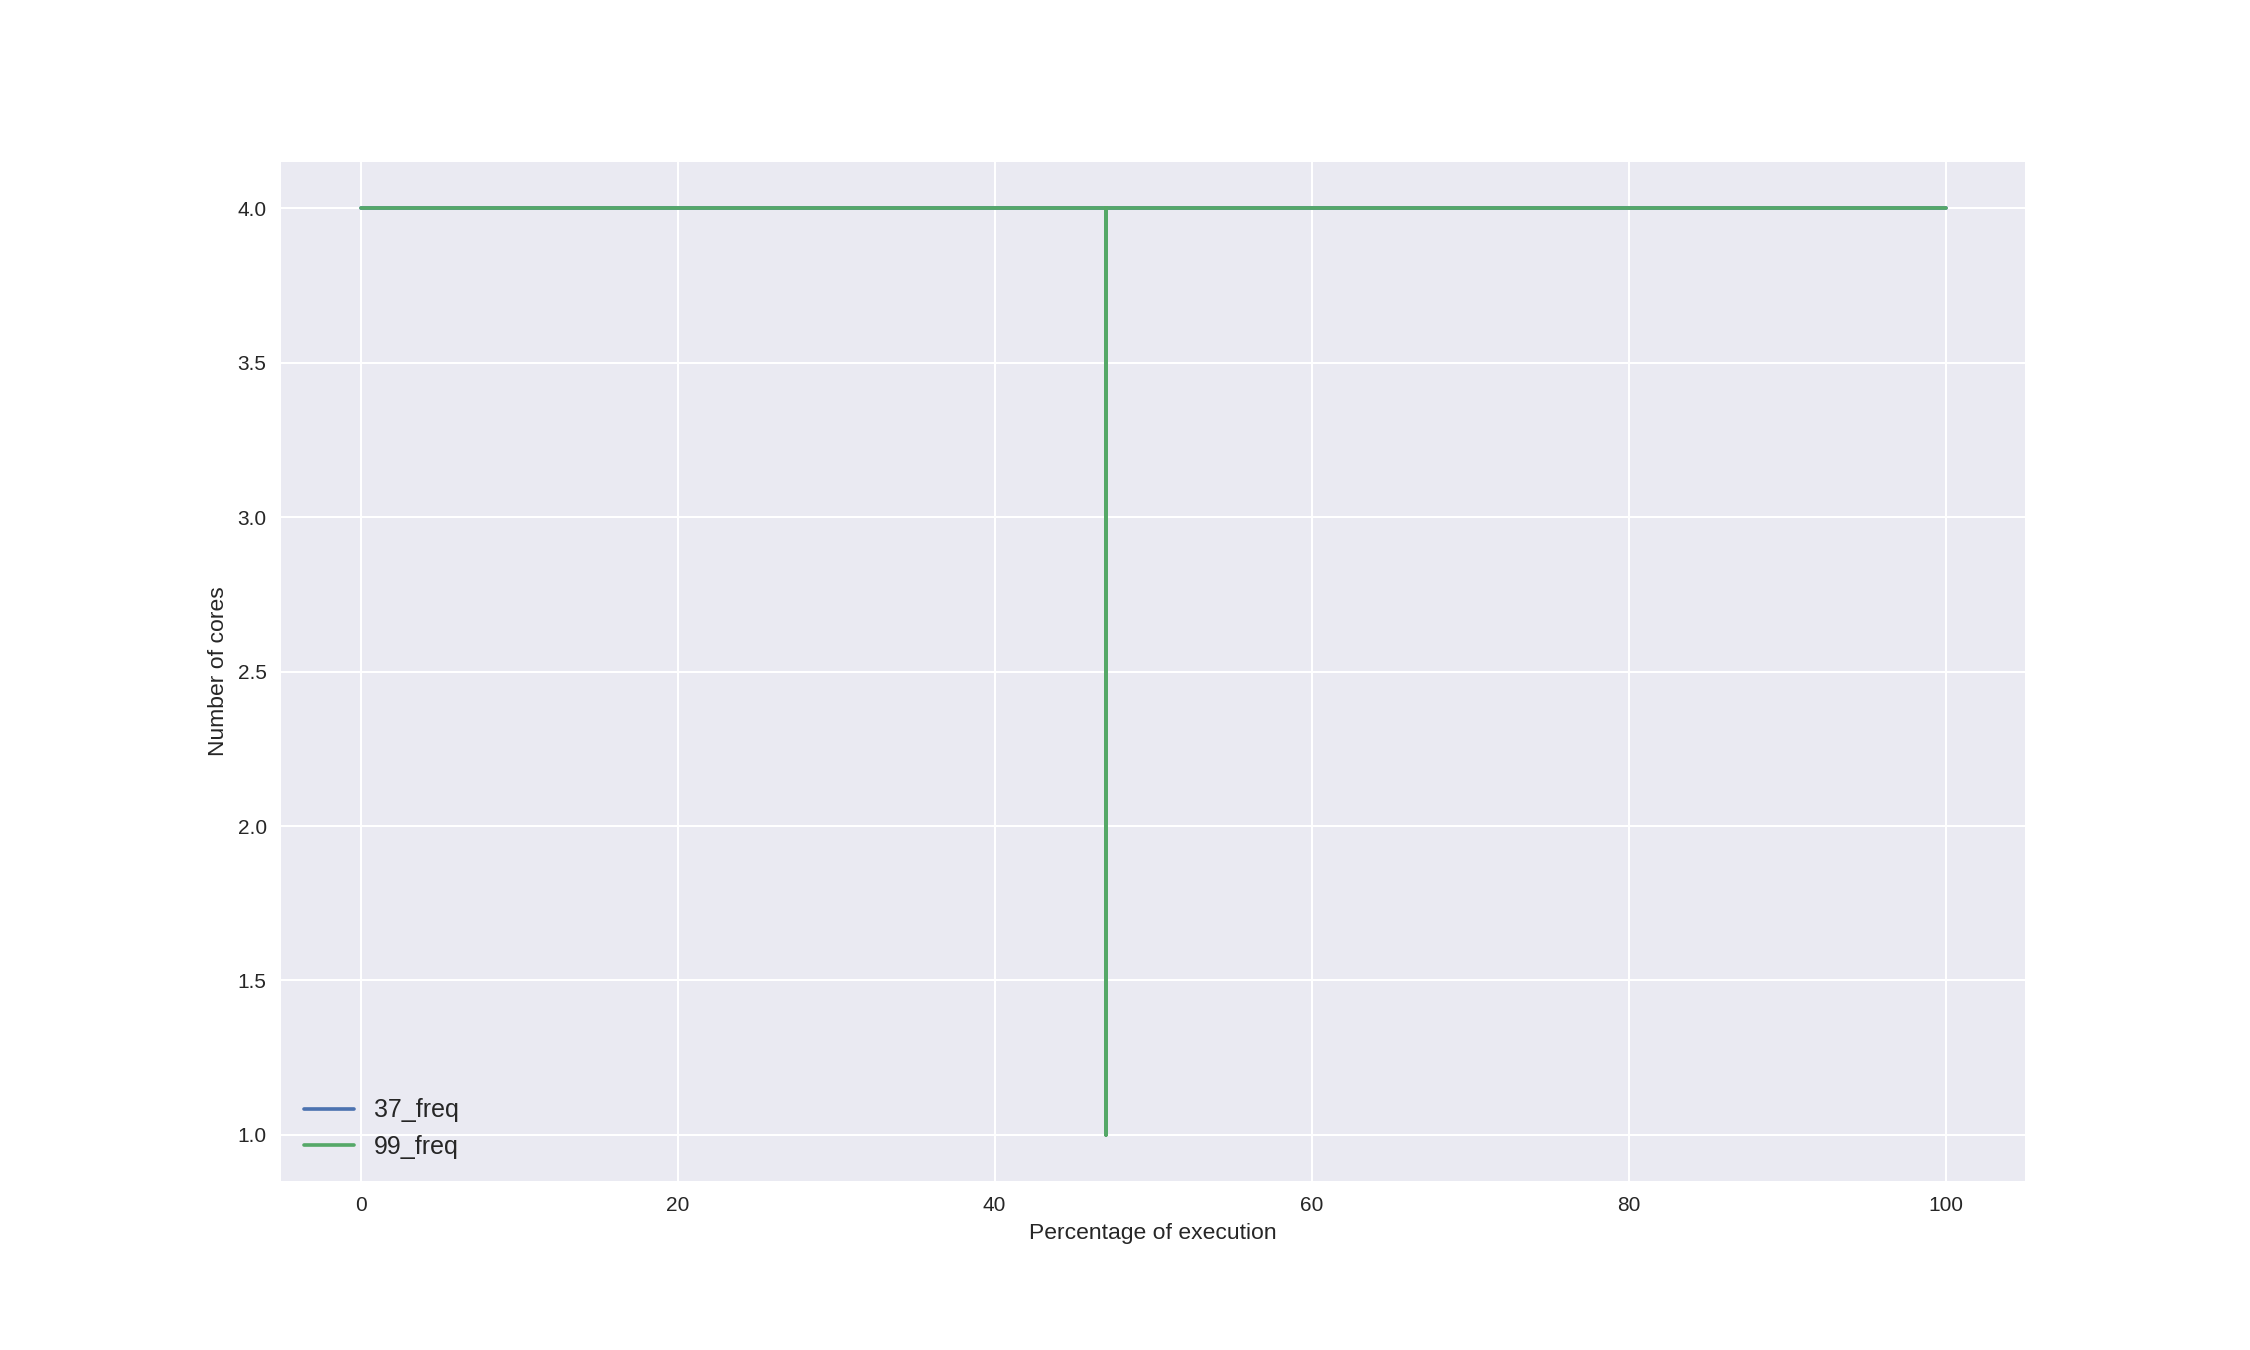
\includegraphics[width=\columnwidth]{phases/figures/signals/completo_canneal_4_cores_signals_cmp.png}  
\caption{Energy and number of cores with 37 and 99 phases.}
    \label{fig:cores_control}
\end{figure}

We observed a similar behavior just considering frequency control energy optimisation (figure \ref{fig:freq_control}).

\begin{figure}[h!]
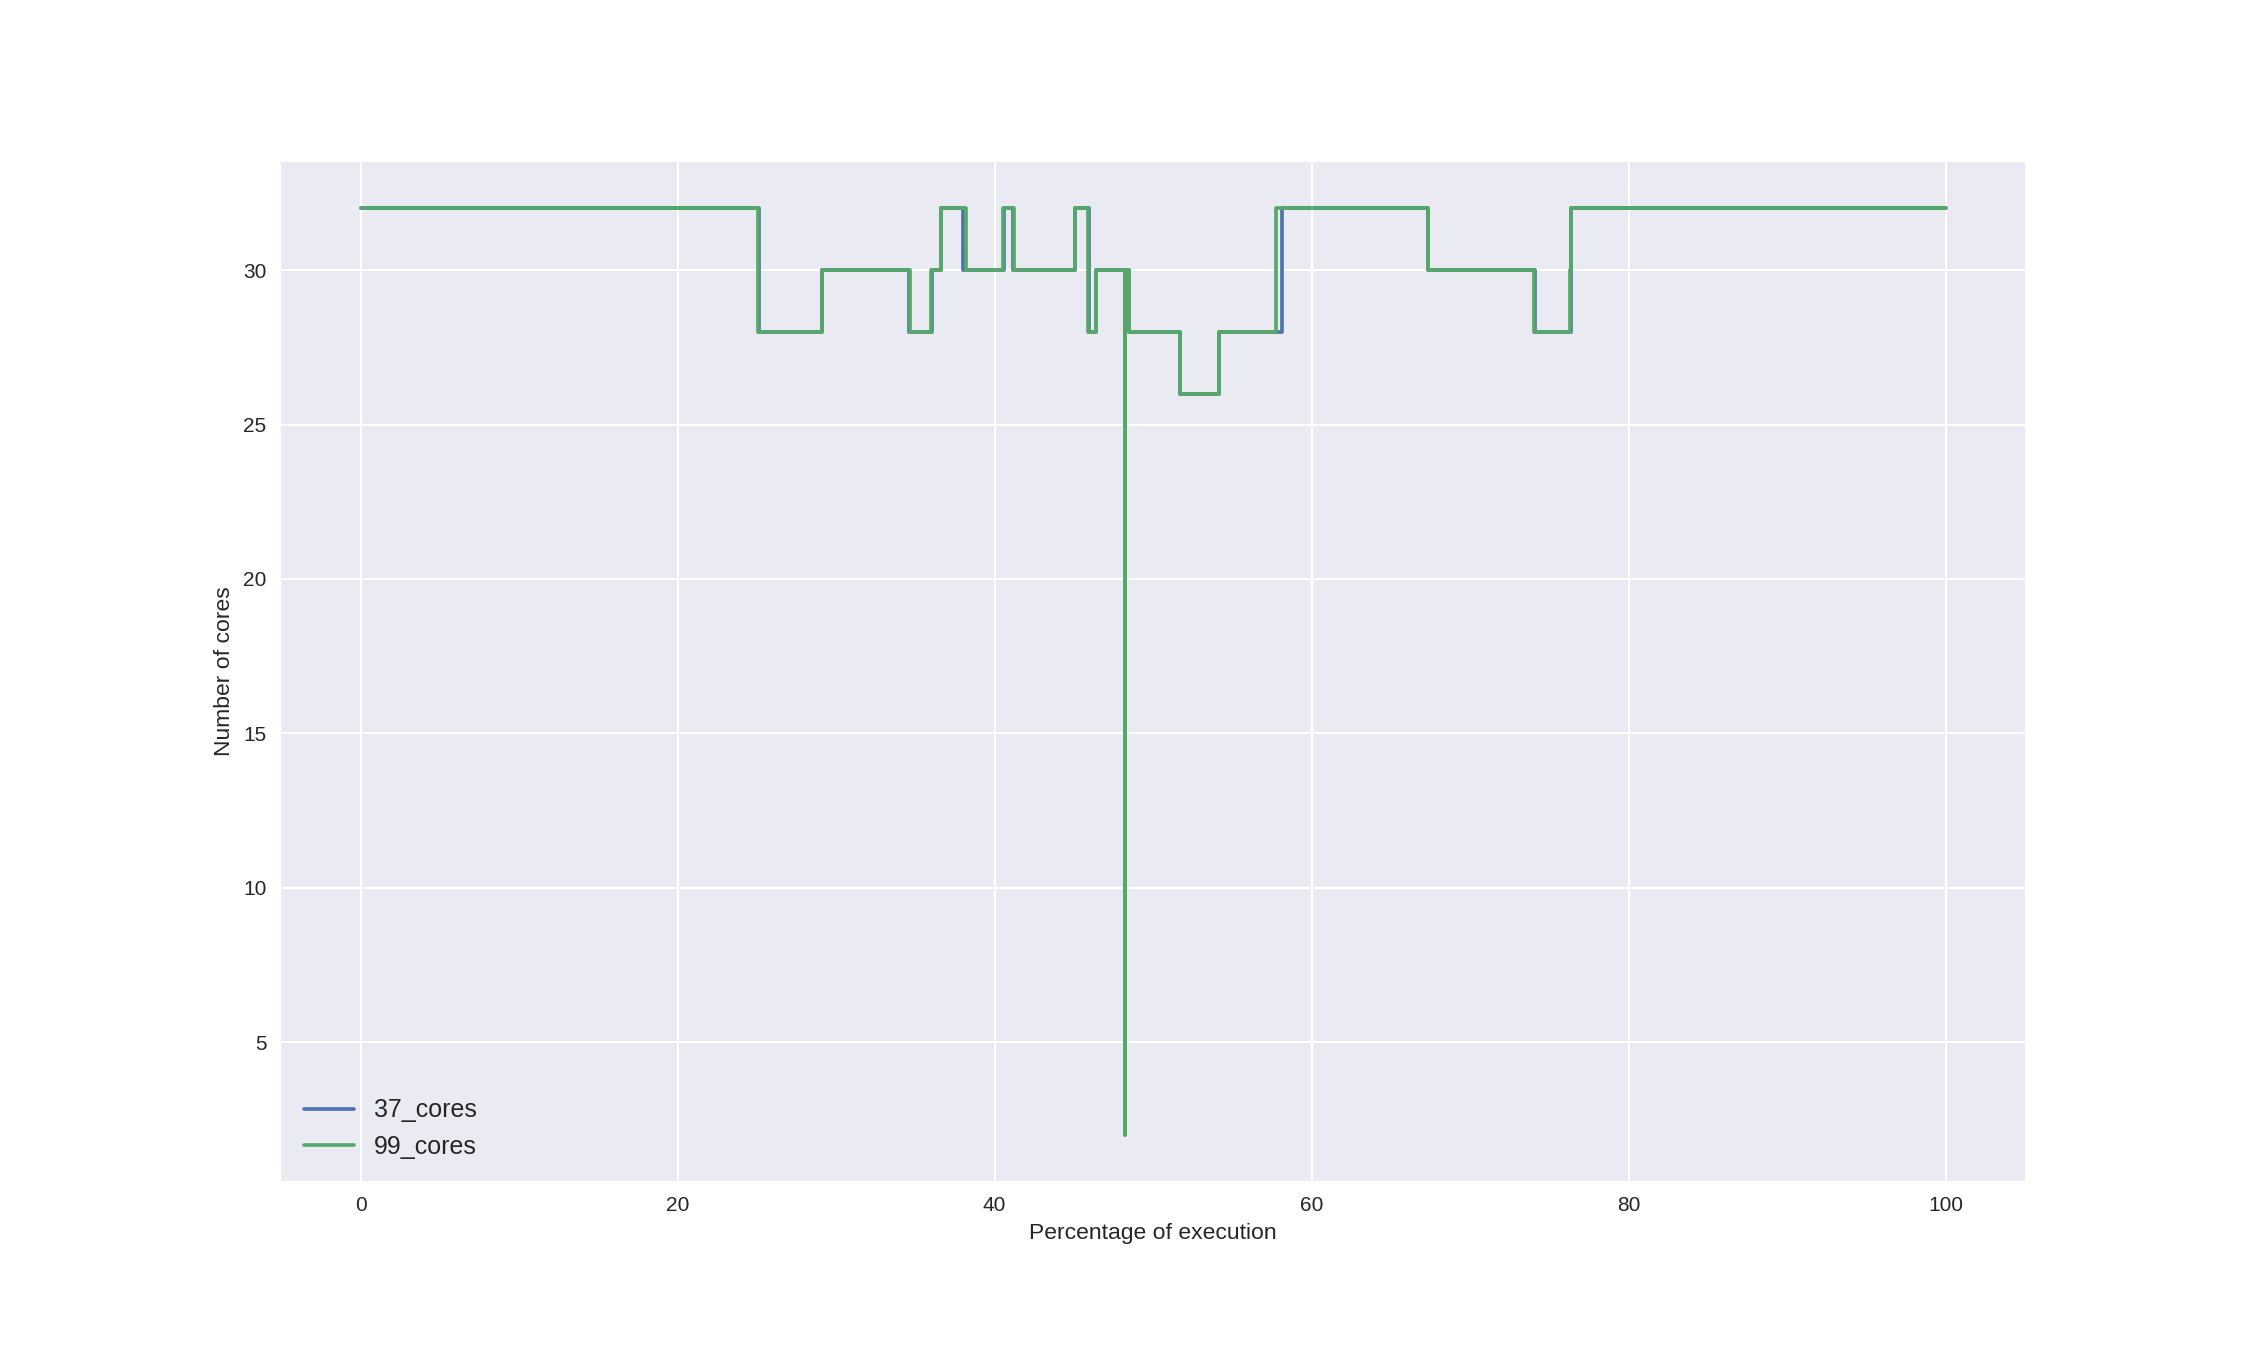
\includegraphics[width=\columnwidth]{phases/figures/signals/completo_black_3_freq_signals_cmp.png}
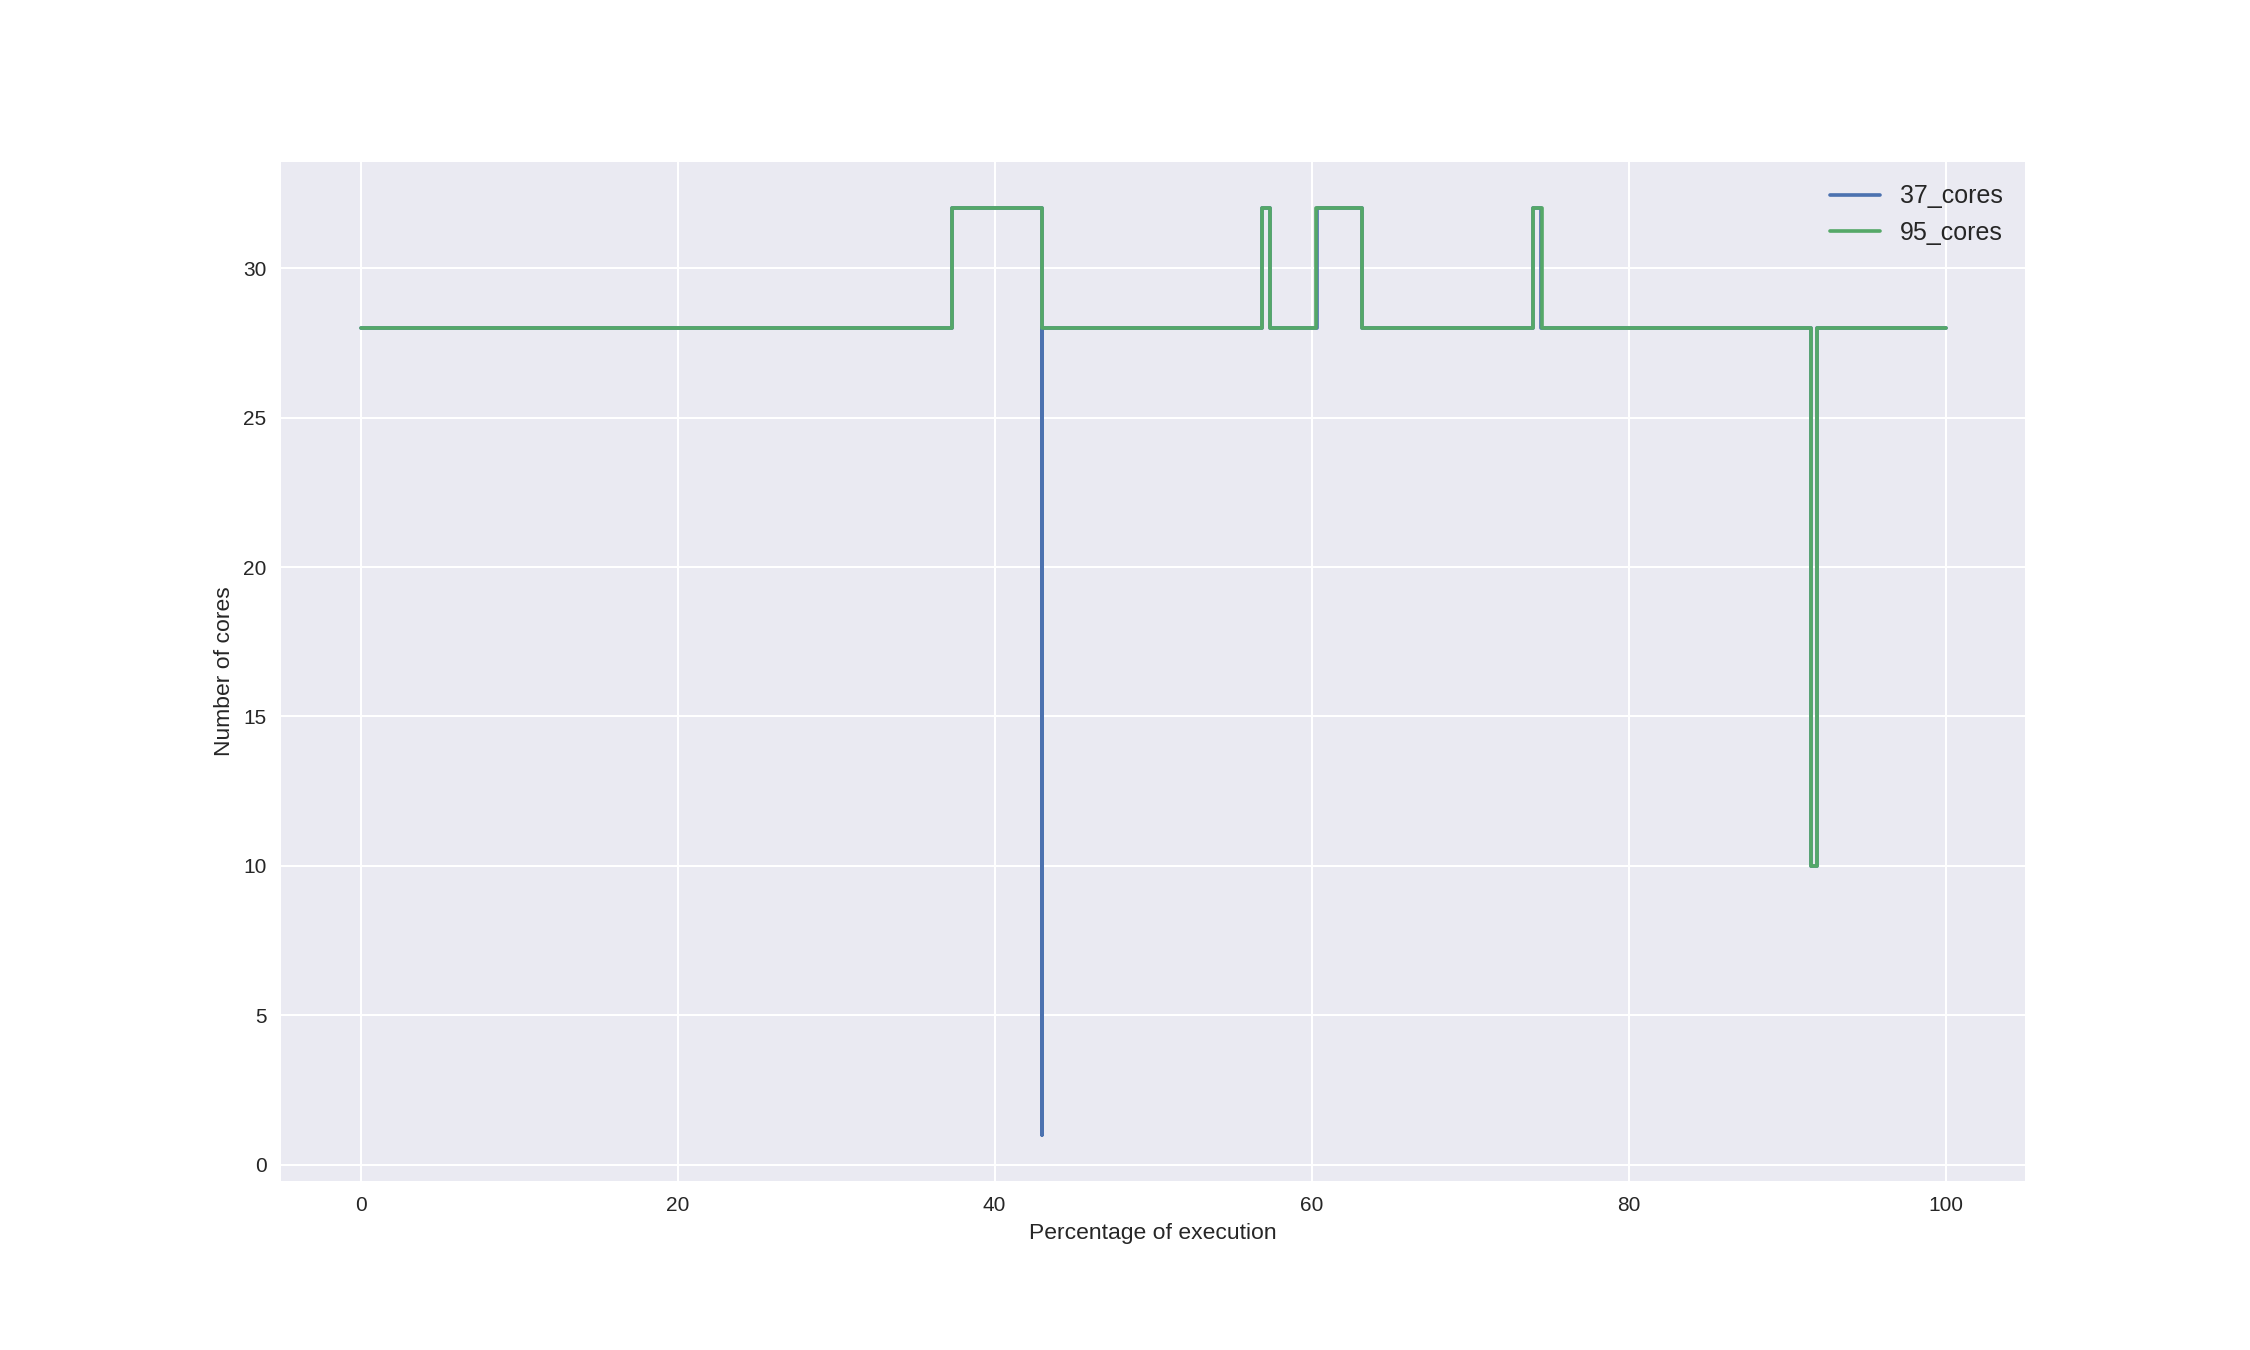
\includegraphics[width=\columnwidth]{phases/figures/signals/completo_bodytrack_3_freq_signals_cmp.png}
%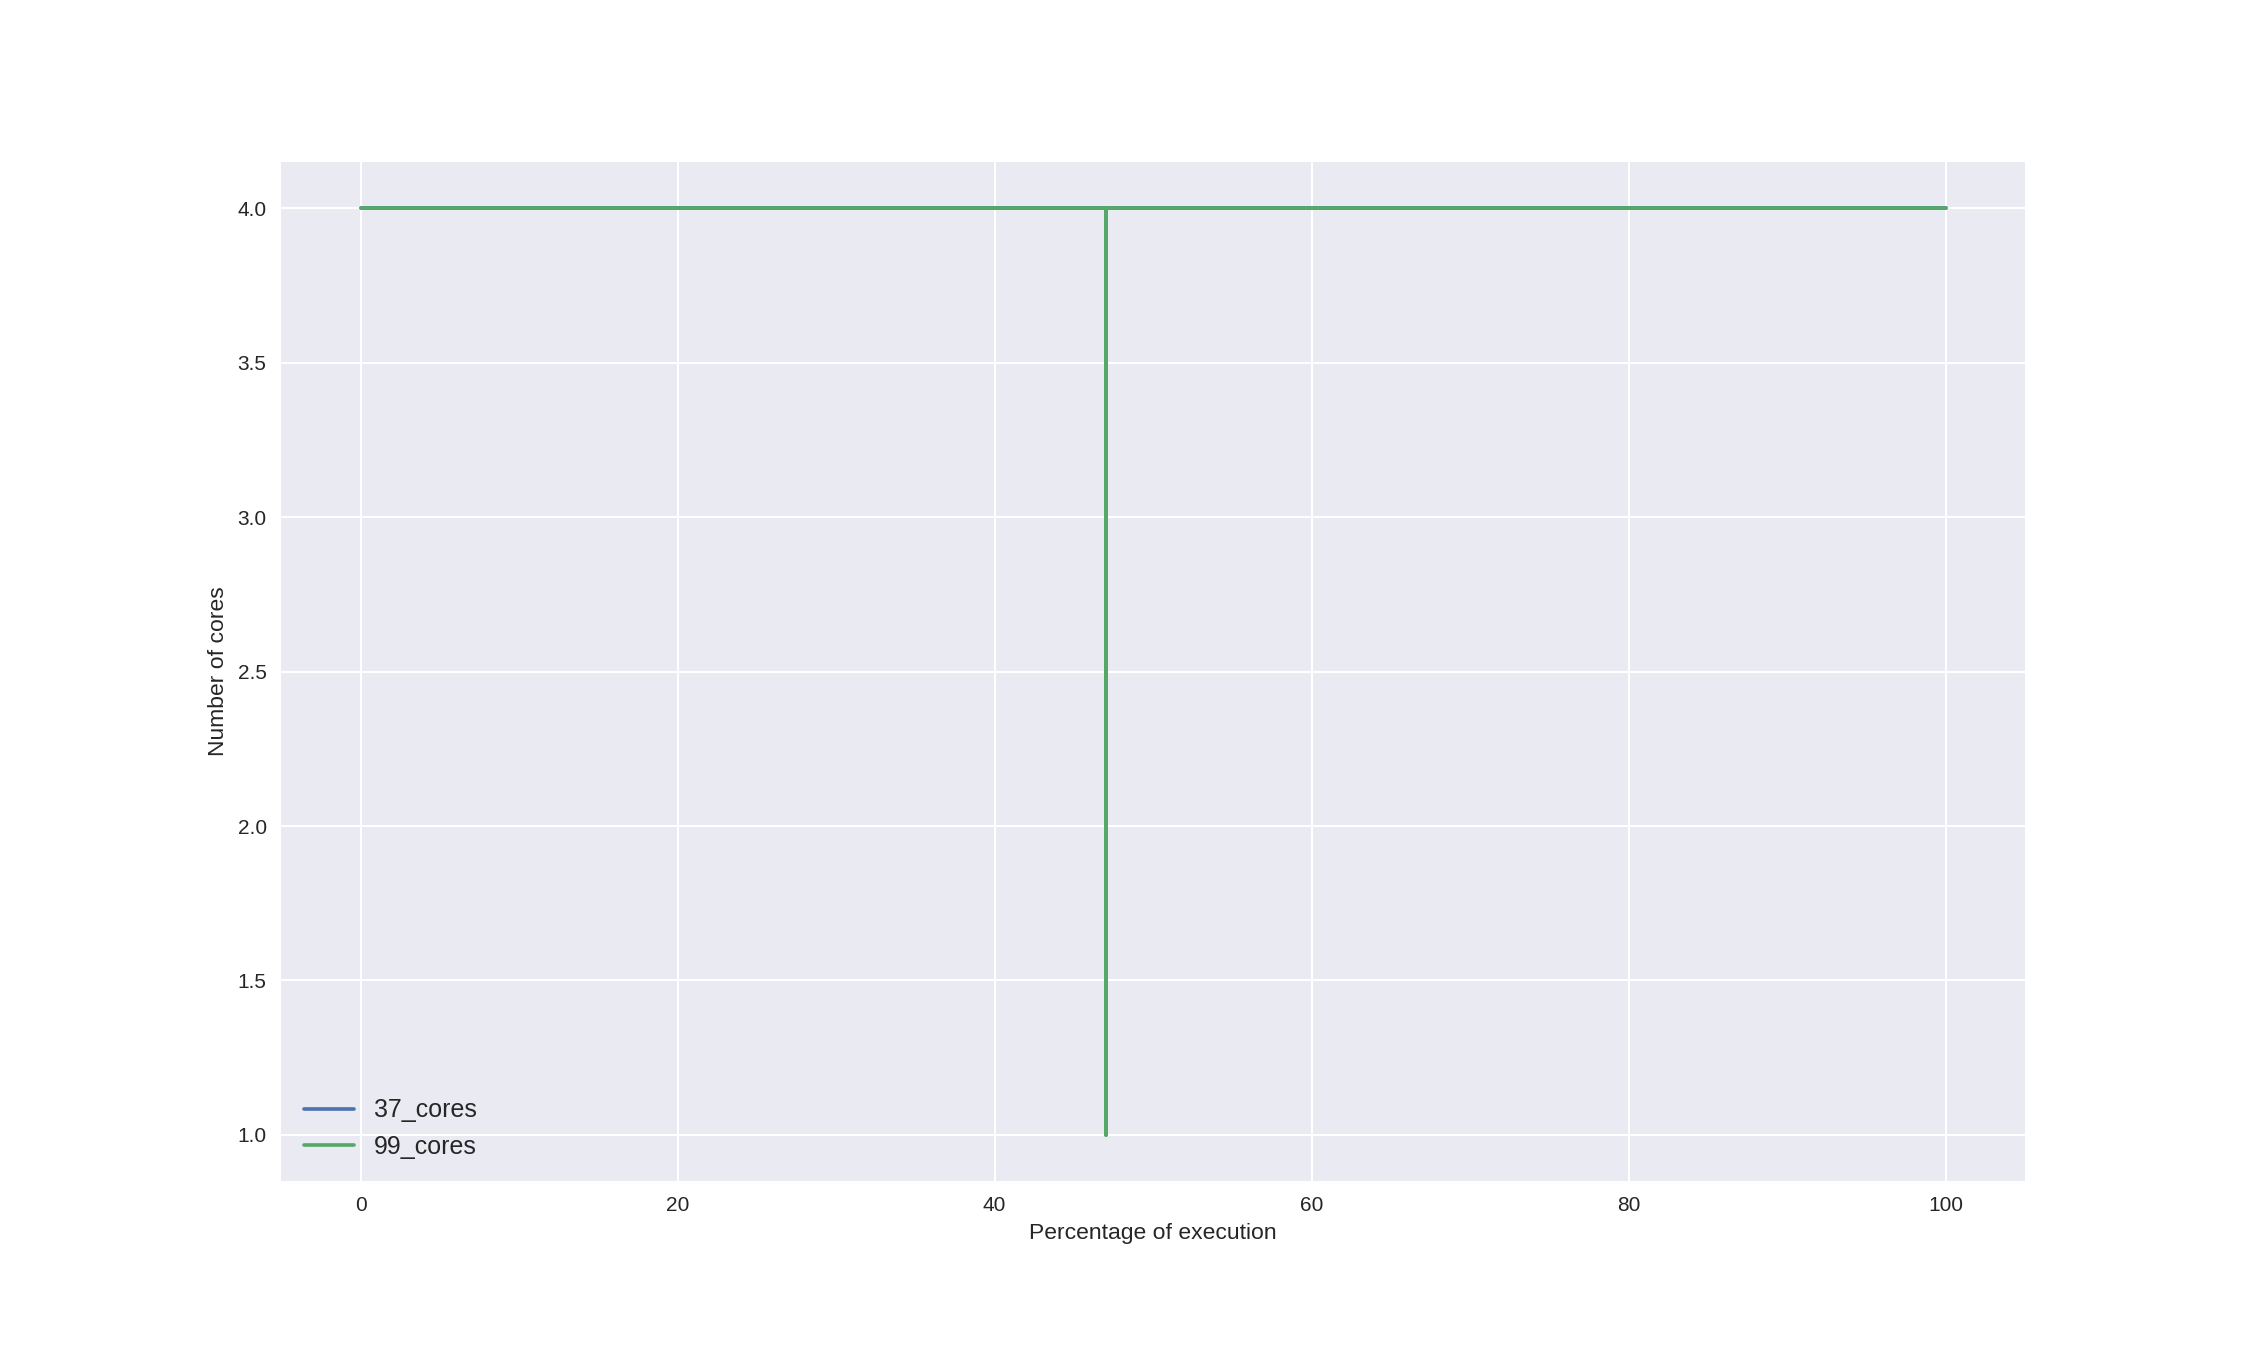
\includegraphics[width=\columnwidth]{phases/figures/signals/completo_canneal_4_freq_signals_cmp.png}
\caption{Energy and frequency with 37 and 99 phases.}
    \label{fig:freq_control}
\end{figure}

The images below show the phases for all applications:
\begin{figure}[H]
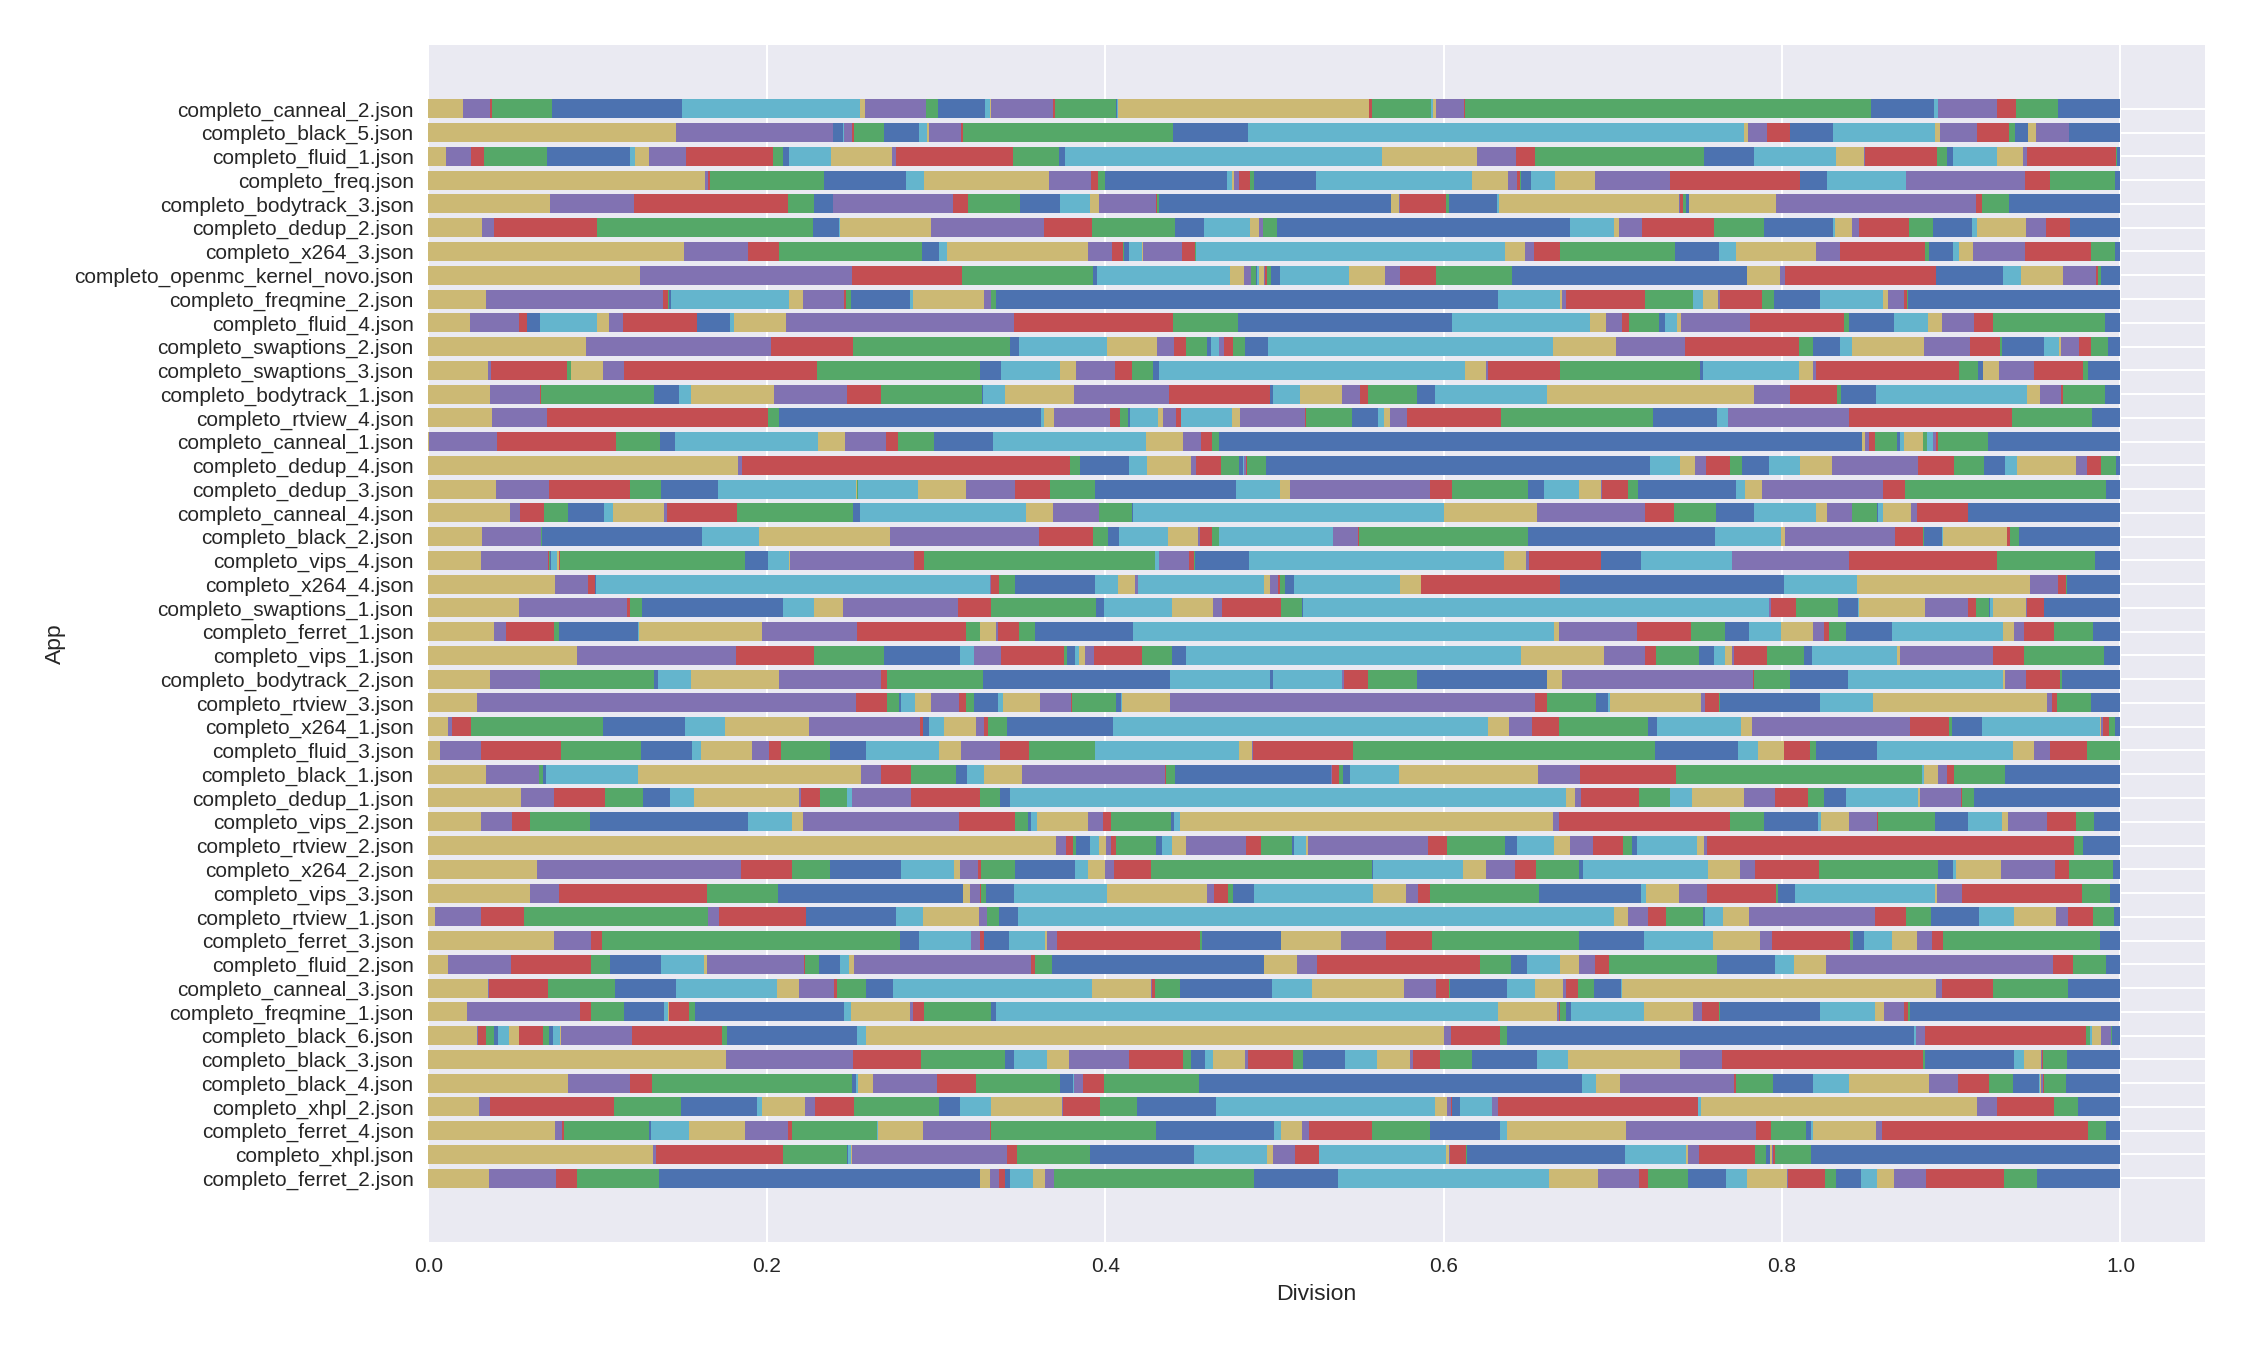
\includegraphics[width=\columnwidth]{phases/figures/phase_division_35.png}
\end{figure}
In most applications, we can see a pattern of 3 phases wich for this applications are generally, and setup phase where it loads data from the disk, a computation phase where the data is processed, and a finalization phase where data is written back to the disk or display to the user.

\begin{figure}[H]
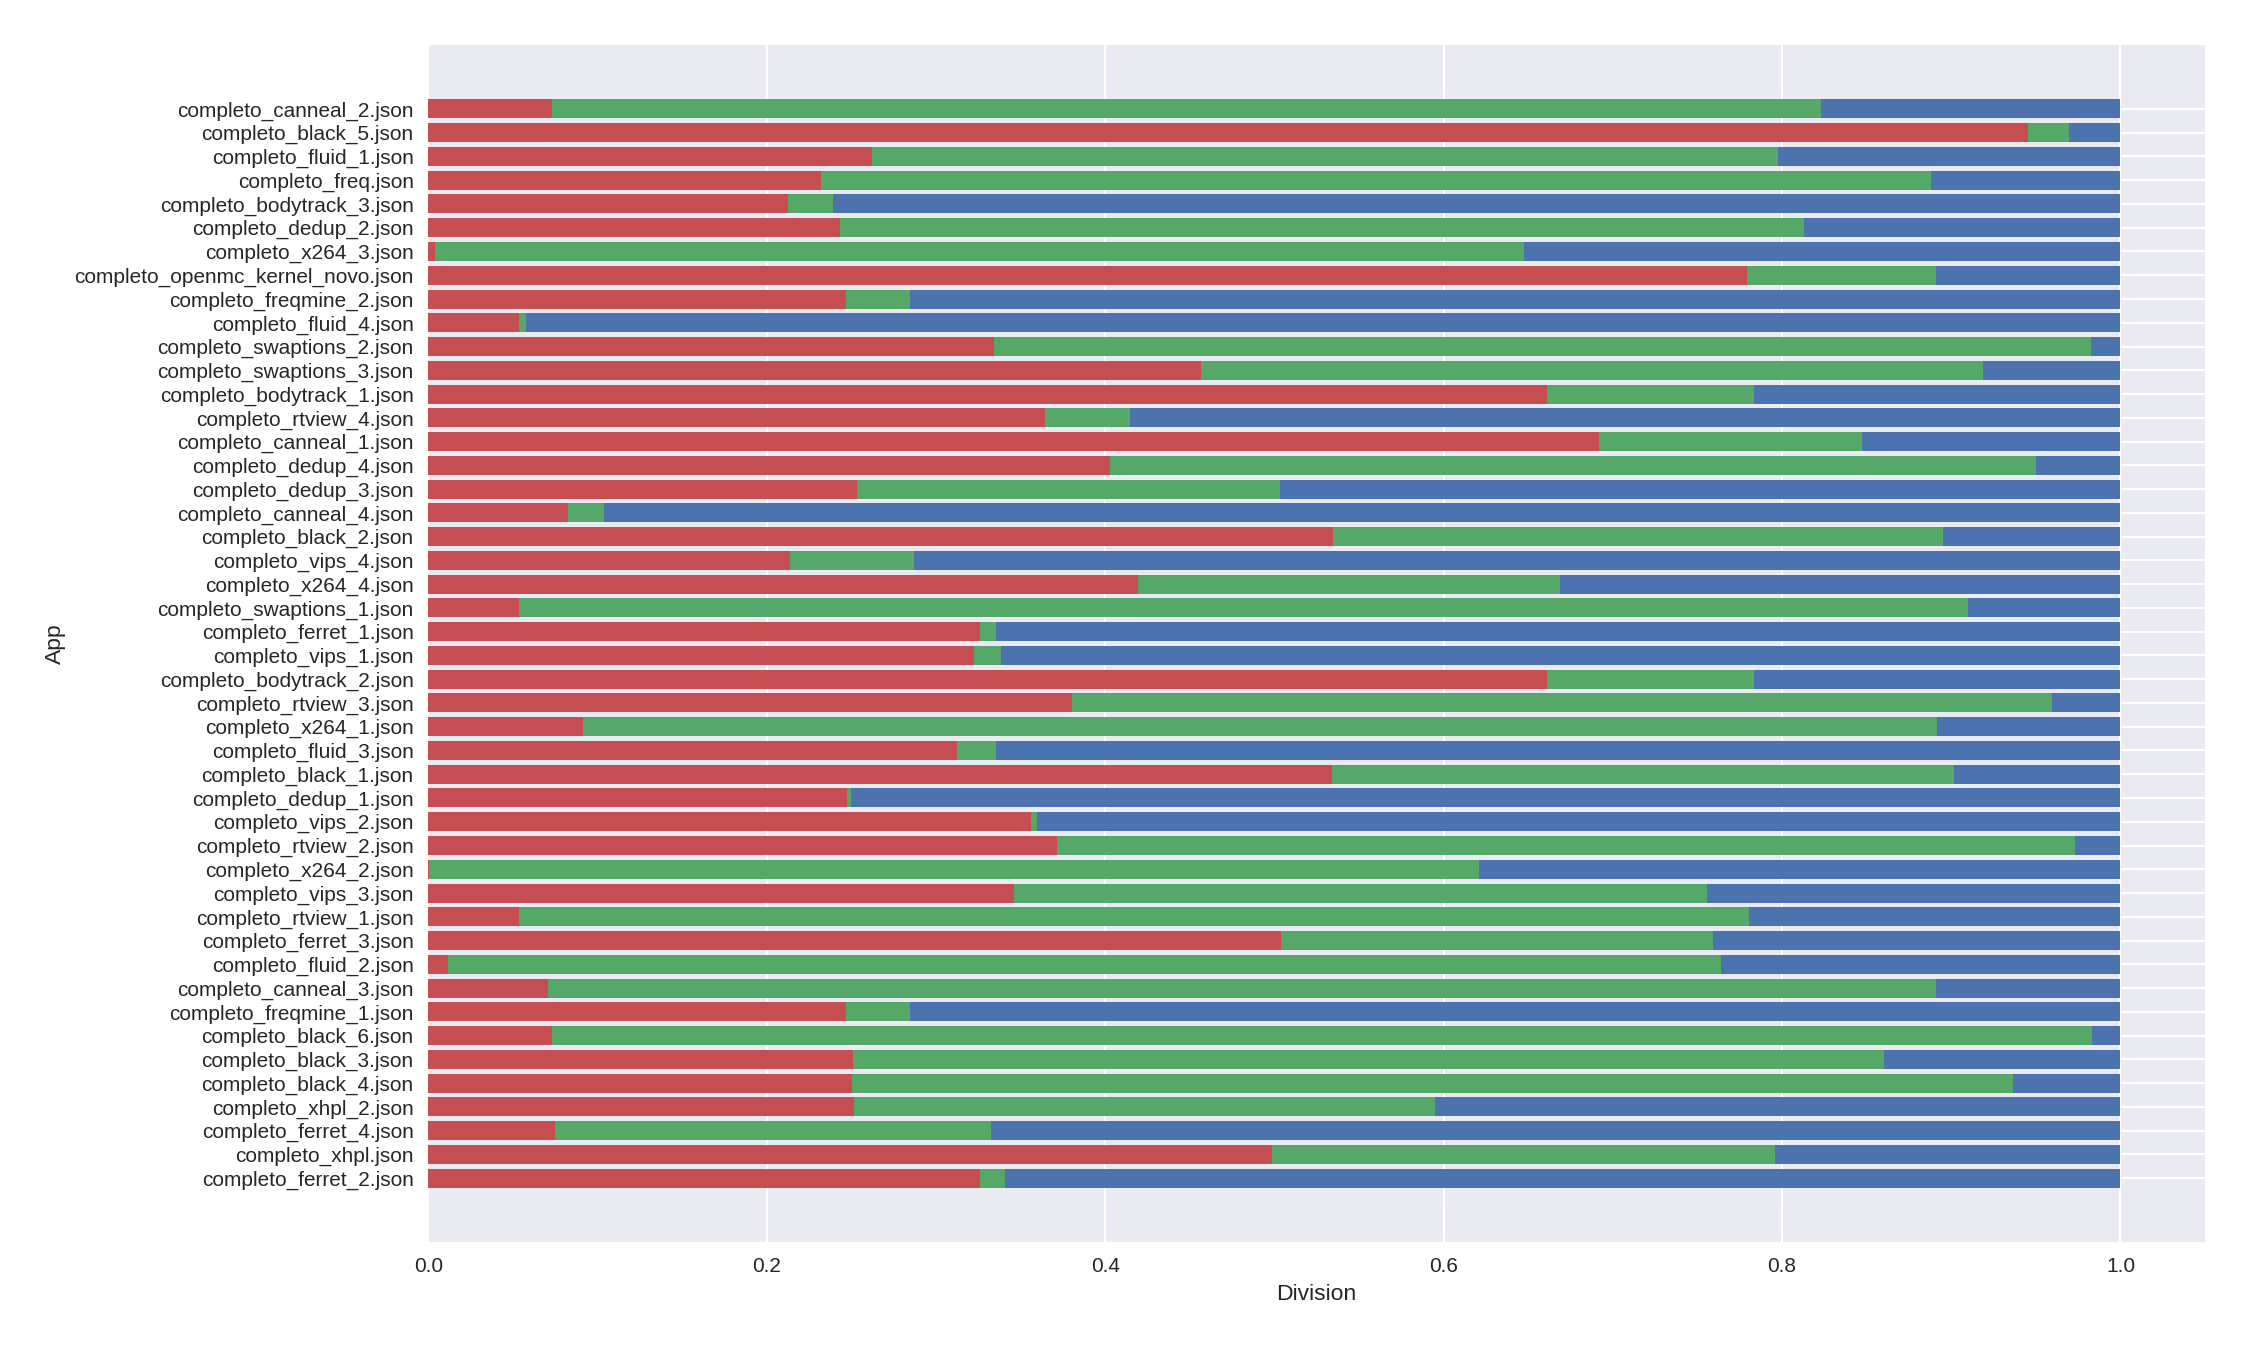
\includegraphics[width=\columnwidth]{phases/figures/phase_division_3.png}
\end{figure}
Plotting for 3 phases, we can observe that better.